% Figure from MATH 556 notes, section 3. Compile with the notes preamble.
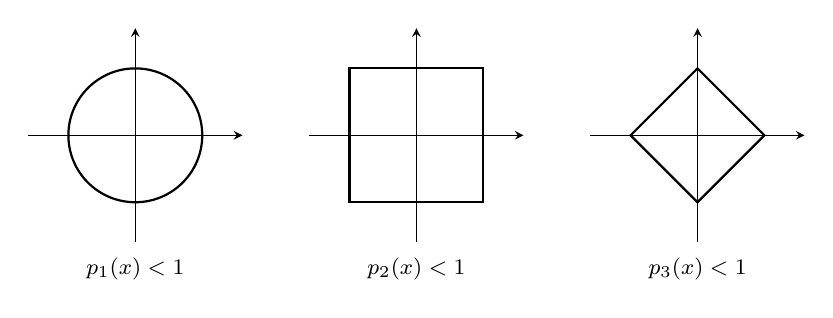
\begin{tikzpicture}[scale=0.85, >=stealth]
    % disk
    \begin{scope}
        \draw[->] (-1.6,0) -- (1.6,0);
        \draw[->] (0,-1.6) -- (0,1.6);
        \draw[thick] (0,0) circle (1);
        \node[font=\footnotesize] at (0,-2) {$p_1(x) < 1$};
    \end{scope}
    % square
    \begin{scope}[xshift=4.2cm]
        \draw[->] (-1.6,0) -- (1.6,0);
        \draw[->] (0,-1.6) -- (0,1.6);
        \draw[thick] (-1,-1) rectangle (1,1);
        \node[font=\footnotesize] at (0,-2) {$p_2(x) < 1$};
    \end{scope}
    % diamond
    \begin{scope}[xshift=8.4cm]
        \draw[->] (-1.6,0) -- (1.6,0);
        \draw[->] (0,-1.6) -- (0,1.6);
        \draw[thick] (1,0) -- (0,1) -- (-1,0) -- (0,-1) -- cycle;
        \node[font=\footnotesize] at (0,-2) {$p_3(x) < 1$};
    \end{scope}
\end{tikzpicture}
